\documentclass[11pt]{article}

% Packages for formatting and aesthetics
\usepackage[utf8]{inputenc}
\usepackage[margin=1in]{geometry}
\usepackage{amsmath, amssymb}
\usepackage{xcolor}
\usepackage{listings}
\usepackage{tcolorbox}
\usepackage[numbers,sort&compress]{natbib}
\usepackage{hyperref}
\usepackage{booktabs}
\usepackage{fancyhdr}
\usepackage{titlesec}

\hypersetup{
    colorlinks=true,       % false: boxed links; true: colored links
    linkcolor=blue,        % color of internal links (sections, figures, tables)
    citecolor=blue,        % color of links to bibliography
    urlcolor=blue          % color of external URLs
}

% Color palette
\definecolor{codebg}{RGB}{245, 247, 250}
\definecolor{codeframe}{RGB}{210, 215, 220}
\definecolor{keywordcolor}{RGB}{0, 102, 204}
\definecolor{commentcolor}{RGB}{100, 110, 120}
\definecolor{stringcolor}{RGB}{180, 50, 50}
\definecolor{accentcolor}{RGB}{40, 90, 150}

% R Code Listing Style
\lstdefinestyle{Rstyle}{
    language=R,
    backgroundcolor=\color{codebg},
    frame=single,
    rulecolor=\color{codeframe},
    basicstyle=\ttfamily\small,
    keywordstyle=\color{keywordcolor}\bfseries,
    commentstyle=\color{commentcolor}\itshape,
    stringstyle=\color{stringcolor},
    numbers=left,
    numberstyle=\tiny\color{commentcolor},
    stepnumber=1,
    numbersep=8pt,
    showstringspaces=false,
    breaklines=true,
    tabsize=2,
    captionpos=b
}
\lstset{style=Rstyle}

% Header and Footer
\pagestyle{fancy}
\fancyhf{}
\lhead{\textbf{Data Mining Lab:} Frequent Patterns \& Association Rules in R}
\rhead{\thepage}
\renewcommand{\headrulewidth}{0.4pt}

% Section styling
\titleformat{\section}{\large\bfseries\color{accentcolor}}{\thesection.}{0.5em}{}[\titlerule]
\titleformat{\subsection}{\normalsize\bfseries\color{accentcolor!80!black}}{\thesubsection}{0.5em}{}

% Custom Callout Boxes
\newtcolorbox{missionbox}[1]{
    colback=blue!5!white,
    colframe=accentcolor,
    fonttitle=\bfseries,
    title=#1
}

\newtcolorbox{trapbox}[1]{
    colback=red!5!white,
    colframe=red!75!black,
    fonttitle=\bfseries,
    title=#1
}

\title{\vspace{-1cm}\textbf{\LARGE The Supermarket Detective:\\ Uncovering Hidden Shopping Habits with R}\\[0.2cm]
\large A Hands-On Lab with \texttt{arules} and \texttt{arulesViz}}
\author{Andrés Oswaldo Calderón Romero}
\date{\today}

\begin{document}

\maketitle

\section{Introuduction}
Welcome, ML Detective! Every day, thousands of customers walk into supermarkets, toss items into their carts, and leave behind a trail of digital breadcrumbs: \textbf{receipts}.  Store managers want to know what is really going on in those aisles. Do people who buy diapers really buy beer? Are folks buying whole milk out of genuine love for dairy, or just because literally everyone buys milk?

In this lab, you will use R's \texttt{arules} and \texttt{arulesViz} packages to interrogate real point-of-sale transaction data, expose misleading patterns, and rearrange the store shelves for maximum profit.

\section{Setting Up Your Detective Toolkit}

Before we can interrogate the data, we need to load our equipment. The \texttt{arules} package \cite{hahsler2005arules, hahsler2011arules} gives us the classic mining algorithms, while \texttt{arulesViz} \cite{hahsler2017arulesviz} turns dry rule tables into interactive networks and plots.

Open RStudio, create a new script, and run the following setup code:

\begin{lstlisting}[caption={Installing and loading the required packages.}]
# Possible dependencies for arulesViz (run once)
# install.packages(c("igraph", "tidygraph", "ggraph"))
# Install packages if you haven't already (run once)
# install.packages(c("arules", "arulesViz"))

library(arules)
library(arulesViz)

# Load the famous Groceries dataset (1 month of real-world point-of-sale data)
data("Groceries")
\end{lstlisting}

\section{Crime Scene Investigation: Exploring Transactions}

Unlike standard data frames with neat rows and columns, market basket data is stored as a \textbf{sparse matrix} (class \texttt{transactions}). If a store sells 169 distinct items, most people only buy 4 or 5 at a time, meaning a normal table would be 98\% empty zeroes!

Let's inspect the ``crime scene'' and see what people are actually buying.

\begin{lstlisting}[caption={Inspecting the sparse transaction matrix and top items.}]
# 1. Check the dimensions and density of the dataset
summary(Groceries)

# 2. Peek at the first 5 receipts (transactions)
inspect(Groceries[1:5])

# 3. Check the exact support (frequency) of the first 3 items
itemFrequency(Groceries[, 1:3])

# 4. Plot the Top 15 most popular items in the store
itemFrequencyPlot(Groceries, topN = 15, type = "relative",
                  col = "steelblue", 
                  main = "Top 15 Most Purchased Items",
                  ylab = "Support (Proportion of Receipts)")
\end{lstlisting}

\textbf{Quick Check:} Look at the plot you just generated. Which item is the undisputed king of this grocery store, appearing in over 25\% of all shopping carts? Keep this item in mind, it is going to try to trick us later!

\section{Mining Frequent Itemsets (The Eclat Way)}

In lectures \cite{han2011data}, you saw how \textbf{Apriori} scans the database level-by-level (breadth-first) \cite{agrawal1994fast} and how \textbf{FP-Growth} uses a compact prefix tree (depth-first) \cite{han2000mining}. R's \texttt{arules} also provides \textbf{Eclat} \cite{zaki2000scalable}, another blazing-fast depth-first algorithm that uses vertical transaction ID intersections.

Let's find combinations of at least 2 items that appear together in at least 1\% of all transactions:

\begin{lstlisting}[caption={Mining frequent itemsets using the Eclat algorithm.}]
# Mine frequent itemsets with min_support = 0.01 and at least 2 items
freq_items <- eclat(Groceries, 
                    parameter = list(supp = 0.01, minlen = 2, maxlen = 5))

# Sort by support and inspect the top 10 pairs/groups
inspect(sort(freq_items, by = "support")[1:10])
\end{lstlisting}

\section{Generating Association Rules \& The ``Whole Milk'' Trap}

Frequent itemsets tell us what appears together, but \textbf{Association Rules} ($X \Rightarrow Y$) tell us directionality: \textit{``If a customer puts $X$ in their basket, how likely are they to also grab $Y$?''}

Let's run the Apriori rule engine with a minimum support of $0.005$ (appears in about 50 carts) and a minimum confidence of $0.50$ (50\% conditional probability).

\begin{lstlisting}[caption={Mining association rules and comparing Confidence vs. Lift.}]
# Mine association rules
rules <- apriori(Groceries, 
                 parameter = list(supp = 0.005, conf = 0.50, minlen = 2))

# How many rules did we find?
length(rules)

# Sort by CONFIDENCE and look at the top 5
inspect(sort(rules, by = "confidence")[1:5])
\end{lstlisting}

\begin{trapbox}{The Support-Confidence Trap!}
Look closely at the top rules sorted by \textbf{Confidence}. Notice how almost every single rule points to \texttt{\{whole milk\}} on the Right-Hand Side (RHS)? 

Remember our Basketball \& Cereal lecture example \cite{han2011data}! Because \texttt{whole milk} is bought by $25.5\%$ of \textit{all} customers anyway, almost anything paired with it will naturally have high confidence \cite{brin1997beyond}.

To find \textbf{true correlation}, we must use \textbf{Lift}:
\[
\text{lift}(X, Y) = \frac{c(X \rightarrow Y)}{s(Y)} = \frac{s(X \cup Y)}{s(X) \times s(Y)}
\]
Now let's sort our rules by \textbf{Lift} instead and see how the story changes!
\end{trapbox}

\begin{lstlisting}[caption={Sorting by Lift and removing redundant rules.}]
# Sort by LIFT and inspect the top 5
inspect(sort(rules, by = "lift")[1:5])

# Prune redundant rules (rules that add extra items without improving confidence)
clean_rules <- rules[!is.redundant(rules)]
length(clean_rules)
\end{lstlisting}

\section{Targeted Interrogation: Subsetting Rules}

Suppose the store's Marketing Director barges into your office: \textit{``We have a massive surplus of \textbf{berries} that are about to spoil! And we also want to know what people buy AFTER they pick up \textbf{root vegetables}!''}

You don't need to scroll through hundreds of rules manually. You can interrogate the rules directly using \texttt{subset()}:

\begin{lstlisting}[caption={Targeting specific items on the LHS or RHS.}]
# Question 1: What drives customers to buy berries? (berries on the RHS)
berry_rules <- subset(Groceries_rules <- apriori(Groceries, 
                      parameter = list(supp = 0.002, conf = 0.20)), 
                       subset = rhs %in% "berries" & lift > 2)
inspect(sort(berry_rules, by = "lift"))

# Question 2: If someone grabs root vegetables (LHS), what else do they buy?
veggie_rules <- subset(clean_rules, subset = lhs %in% "root vegetables")
inspect(sort(veggie_rules, by = "lift")[1:5])
\end{lstlisting}

\section{Visualizing the Evidence (\texttt{arulesViz})}

Tables of numbers put store managers to sleep. Let's turn our top rules into visual network maps, scatter plots, and grouped matrices using the visualization framework in \texttt{arulesViz} \cite{hahsler2017arulesviz}.  You can see the results of the last plots in figures \ref{fig:graph} and \ref{fig:grouped}.

\begin{lstlisting}[caption={Visualizing rules with scatter plots, network graphs, and grouped matrices.}]
# 1. Scatter plot of all clean rules (Support vs. Confidence, shaded by Lift)
plot(clean_rules, measure = c("support", "confidence"), shading = "lift", 
     jitter = 0)

# 2. Grab the top 15 rules by Lift for a clean network graph
top15_lift <- head(sort(clean_rules, by = "lift"), 15)

# 3. Plot as a directed network graph (Circles = Lift/Support, Arrows = Rules)
plot(top15_lift, method = "graph", engine = "htmlwidget")

# 4. Grouped Matrix plot (great for spotting clusters of related rules)
plot(clean_rules, method = "grouped")
\end{lstlisting}

\begin{figure}[t]
    \centering
    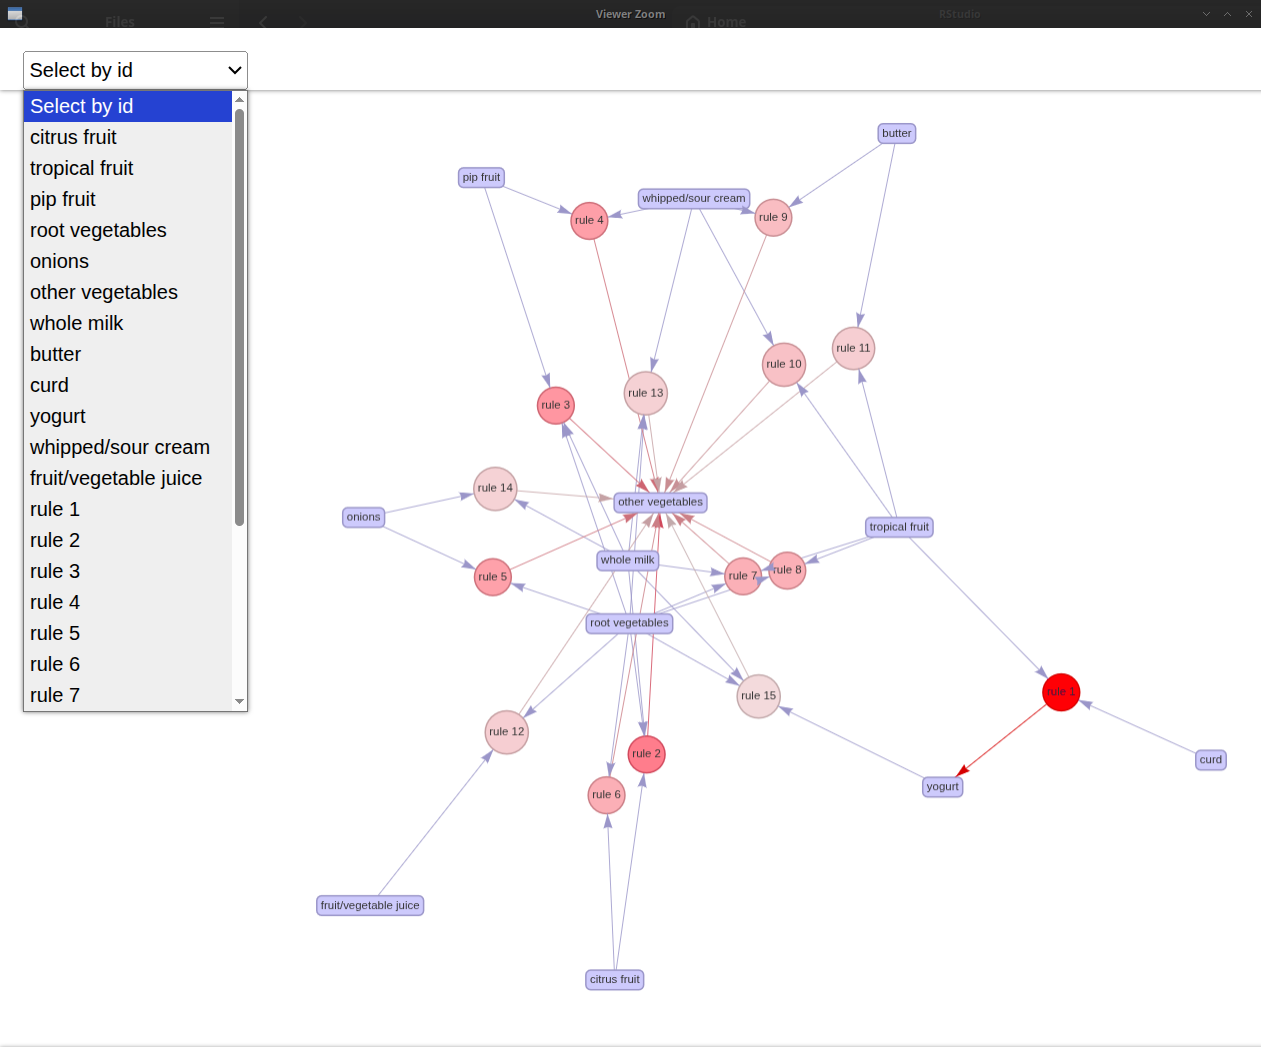
\includegraphics[width=0.6\textwidth]{figures/graph.png}
    \caption{\textbf{Directed Network Graph of the Top 15 Association Rules Ranked by Lift.}
    Items are represented as text nodes and association rules as circular intermediate nodes, with directed arrows pointing from the antecedent (LHS) to the consequent (RHS). The size of each rule circle corresponds to its \textbf{Support} (frequency of occurrence in the dataset), while the color shading intensity represents \textbf{Lift} (strength of positive correlation).}
    \label{fig:graph}
\end{figure}

\begin{figure}[t]
 \centering
 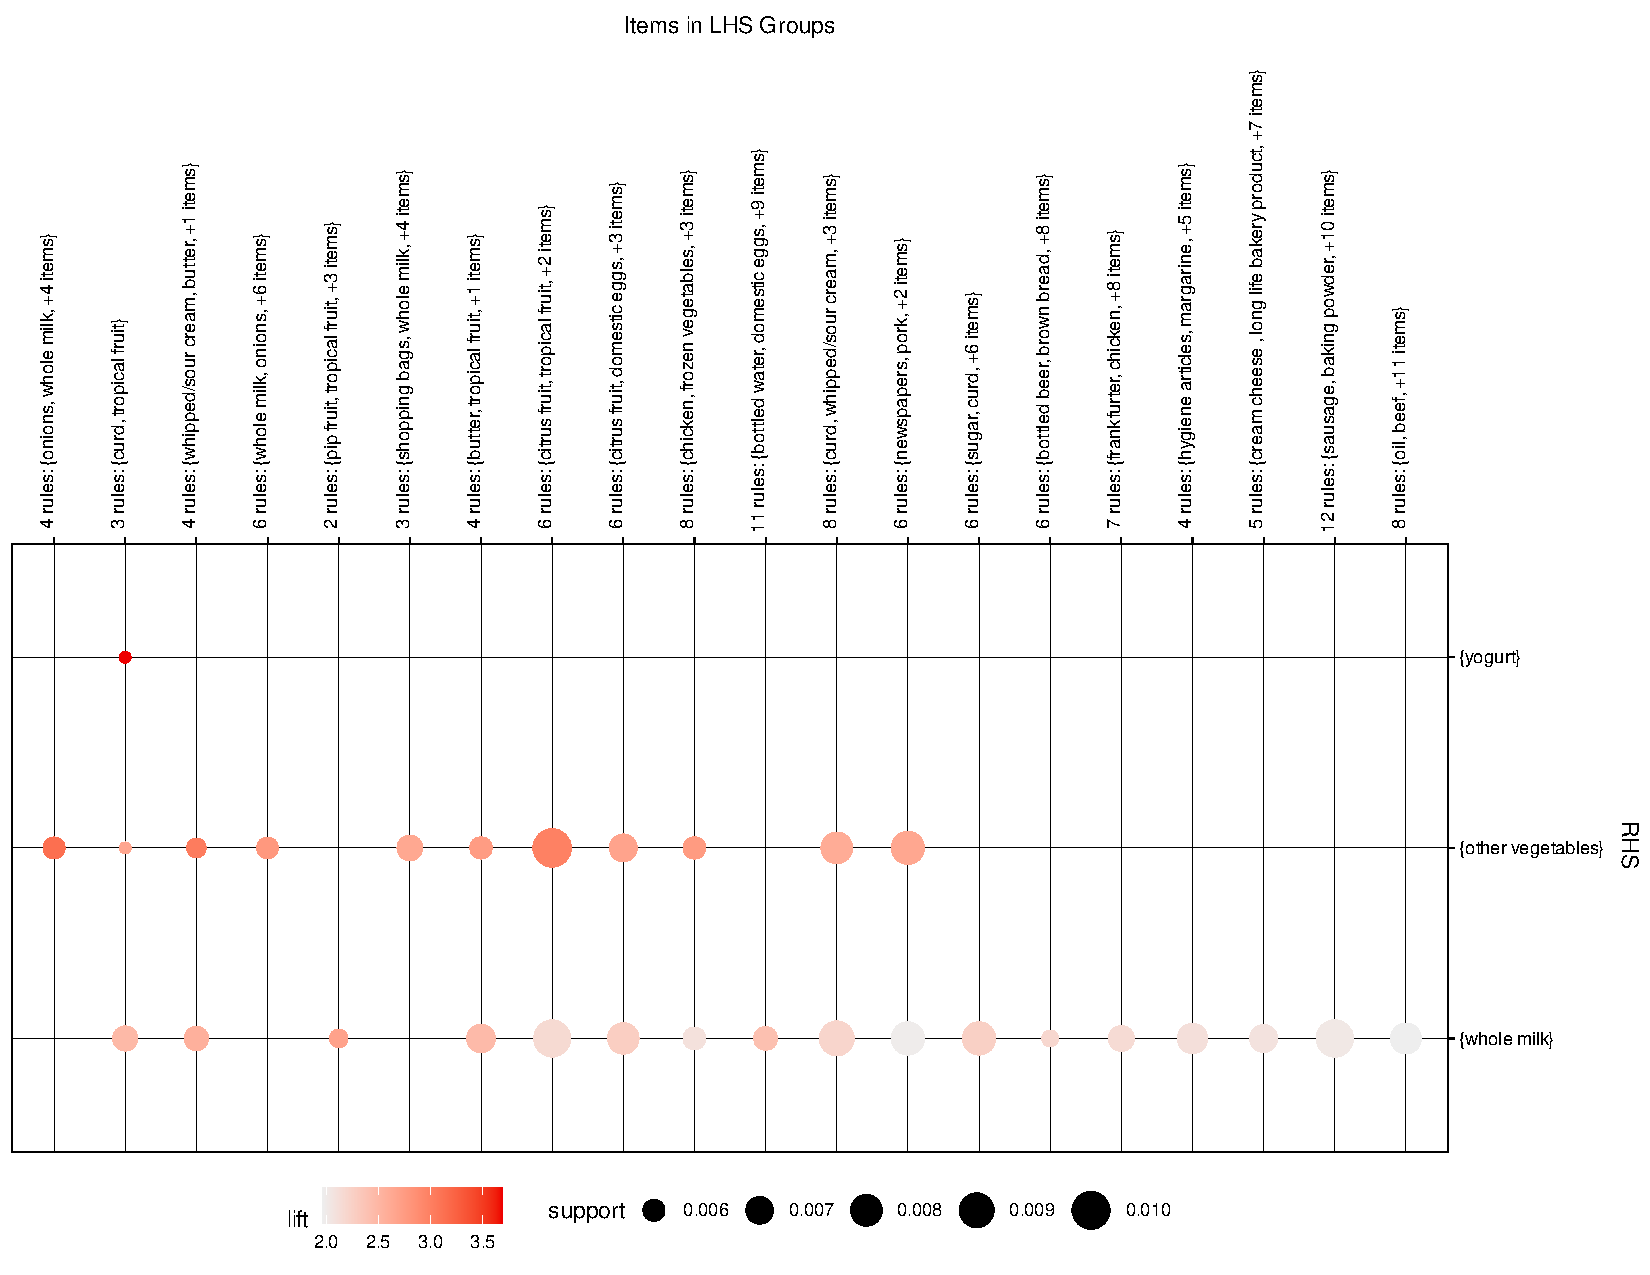
\includegraphics[width=\textwidth]{figures/grouped.pdf}
 \caption{\textbf{Grouped Matrix Visualization of Pruned Association Rules.}
    Antecedent itemsets (LHS, columns) are clustered into $k$ groups based on shared consequent items (RHS, rows). The balloon size at each matrix intersection indicates the aggregated \textbf{Support} of the rules within that cluster, while the color shading reflects the median \textbf{Lift} (darker shades indicate stronger positive associations), ordered from the highest-lift clusters in the top-left to the lowest in the bottom-right.}
 \label{fig:grouped}
\end{figure}

\section{Autonomous Work: The Store Manager's Challenge}

Now it is time to take off the training wheels. Complete the following three challenges on your own and submit a short PDF report containing your R code, plots, and written answers.

\subsection*{Challenge 1: The Beer \& Bottled Water Showdown}
Store folklore says that people buying \texttt{bottled beer} have totally different snack habits than people buying \texttt{soda}.
\begin{enumerate}
    \item Mine association rules from \texttt{Groceries} using a lower support threshold ($\text{supp} = 0.001$, $\text{conf} = 0.15$) so you can catch niche patterns.
    \item Extract two subsets of rules: one where \texttt{bottled beer} is on the LHS, and one where \texttt{soda} is on the LHS.
    \item Compare the top 5 rules (sorted by \textbf{Lift}) for each drink. What is the most surprising item positively correlated with \texttt{bottled beer}?
\end{enumerate}

\subsection*{Challenge 2: Hunting for Negative Correlations ($\text{Lift} < 1$)}
Throughout the lab, we set high confidence thresholds, which naturally filtered out negatively correlated items.
\begin{enumerate}
    \item Run \texttt{apriori()} with $\text{supp} = 0.01$ and a very low confidence ($\text{conf} = 0.05$, $\text{minlen} = 2$).
    \item Filter the rules using \texttt{subset()} to find rules where $\text{lift} < 0.75$.
    \item Pick the pair with the lowest lift. Verify the Lift value \textbf{by hand} (or using basic R math) from the individual supports of the LHS, RHS, and their union, just like we did in the lecture slides! Explain in plain language why these two items repel each other.
\end{enumerate}

\subsection*{Challenge 3: The ``Adult'' Census Investigation (Beyond Groceries!)}
Association rule mining isn't just for supermarkets, it works on any categorical dataset!
\begin{enumerate}
    \item Load the built-in US Census dataset using \texttt{data("Adult")}.
    \item Mine rules that predict high earners by setting the Right-Hand Side appearance to high income:
\begin{lstlisting}
income_rules <- apriori(Adult, 
  parameter = list(supp = 0.02, conf = 0.50),
  appearance = list(rhs = c("income=large"), default = "lhs"))
\end{lstlisting}
    \item Remove redundant rules, sort the remaining rules by \textbf{Lift}, and plot the top 10 rules using \texttt{method = "graph"}.
    \item Write a brief 3-sentence summary explaining which demographic or work factors have the strongest positive correlation with earning a large income, and explain why sorting by \textbf{Lift} gives a better insight here than sorting by \textbf{Support}.
\end{enumerate}

\begin{tcolorbox}[
    colback=blue!5!white,
    colframe=accentcolor,
    title=\textbf{Submission Instructions},
    fonttitle=\bfseries,
    boxrule=0.8pt,
    arc=4mm
]
Compile all your findings regarding these challenges into a well-structured PDF report. Submit your completed report to the corresponding Brightspace\texttrademark assignment by 7:00 PM on November 27, 2026.
\end{tcolorbox}

\section{Conclusion}

Through this investigation, you have moved beyond raw transaction logs to uncover the hidden patterns driving customer behavior. By applying the \texttt{arules} package to sparse market basket data, you experienced firsthand both the power of frequent itemset mining and the classic pitfall of the Support-Confidence framework: the ``whole milk trap''. High support and confidence alone often just highlight store bestsellers rather than genuine relationships, demonstrating why \textbf{Lift} is essential for separating mere coincidence from true positive or negative correlation.

Furthermore, pairing statistical rule mining with \texttt{arulesViz} bridged the gap between thousands of raw mathematical rules and actionable human insight. Whether you are optimizing supermarket shelf layouts, building e-commerce recommendation engines, or analyzing demographic census data, the workflow you mastered today, filtering, pruning redundant rules, evaluating lift, and visualizing rule networks, forms the core foundation of pattern discovery across any domain.

\nocite{*}

\bibliographystyle{plainnat}
\bibliography{Lab04}

\end{document}
